\documentclass{beamer}
\usepackage[utf8]{inputenc}
\usepackage{hyperref}
\usepackage{listings}
\usepackage{subcaption}
\usepackage{amsmath}
\usepackage{mathtools}


\lstdefinestyle{saneCode}{
    belowcaptionskip=1\baselineskip,
    breaklines=true,
    frame=none,
    numbers=none,
    basicstyle=\tiny\ttfamily,
    % keywordstyle=\bfseries\color{green!40!black},
    commentstyle=\itshape\color{purple!40!black},
    % identifierstyle=\color{blue},
    backgroundcolor=\color{gray!10!white},
    keepspaces,
    upquote=true,
    showstringspaces=false,
}

\usetheme{Singapore}
\usecolortheme{default}

\title{Seeing the Unseen with Machine Learning}
\subtitle{A Physics-Informed Neural Network Approach to Inverse Problems}
\author[Thompson, Nameika]{
  Nameika, Michael \\
  \and
  Thompson, Jonathan
}

\institute[UCCS]{University of Colorado at Colorado Springs}

\date[UCCS 2023]
{May 08, 2023}

% \logo{\includegraphics[height=1cm]{overleaf-logo}}

\begin{document}
\beamertemplatenavigationsymbolsempty

% Title Page
\frame{\titlepage}

% Presentation Content
\begin{frame}
    \frametitle{The Problem}

    Given a physical system for which we have some experimental data, can we utilize machine learning to understand the
    physics of the system?
    \bigskip

    \begin{figure}
        \centering
        \begin{subfigure}[b]{0.45\textwidth}
            \centering
            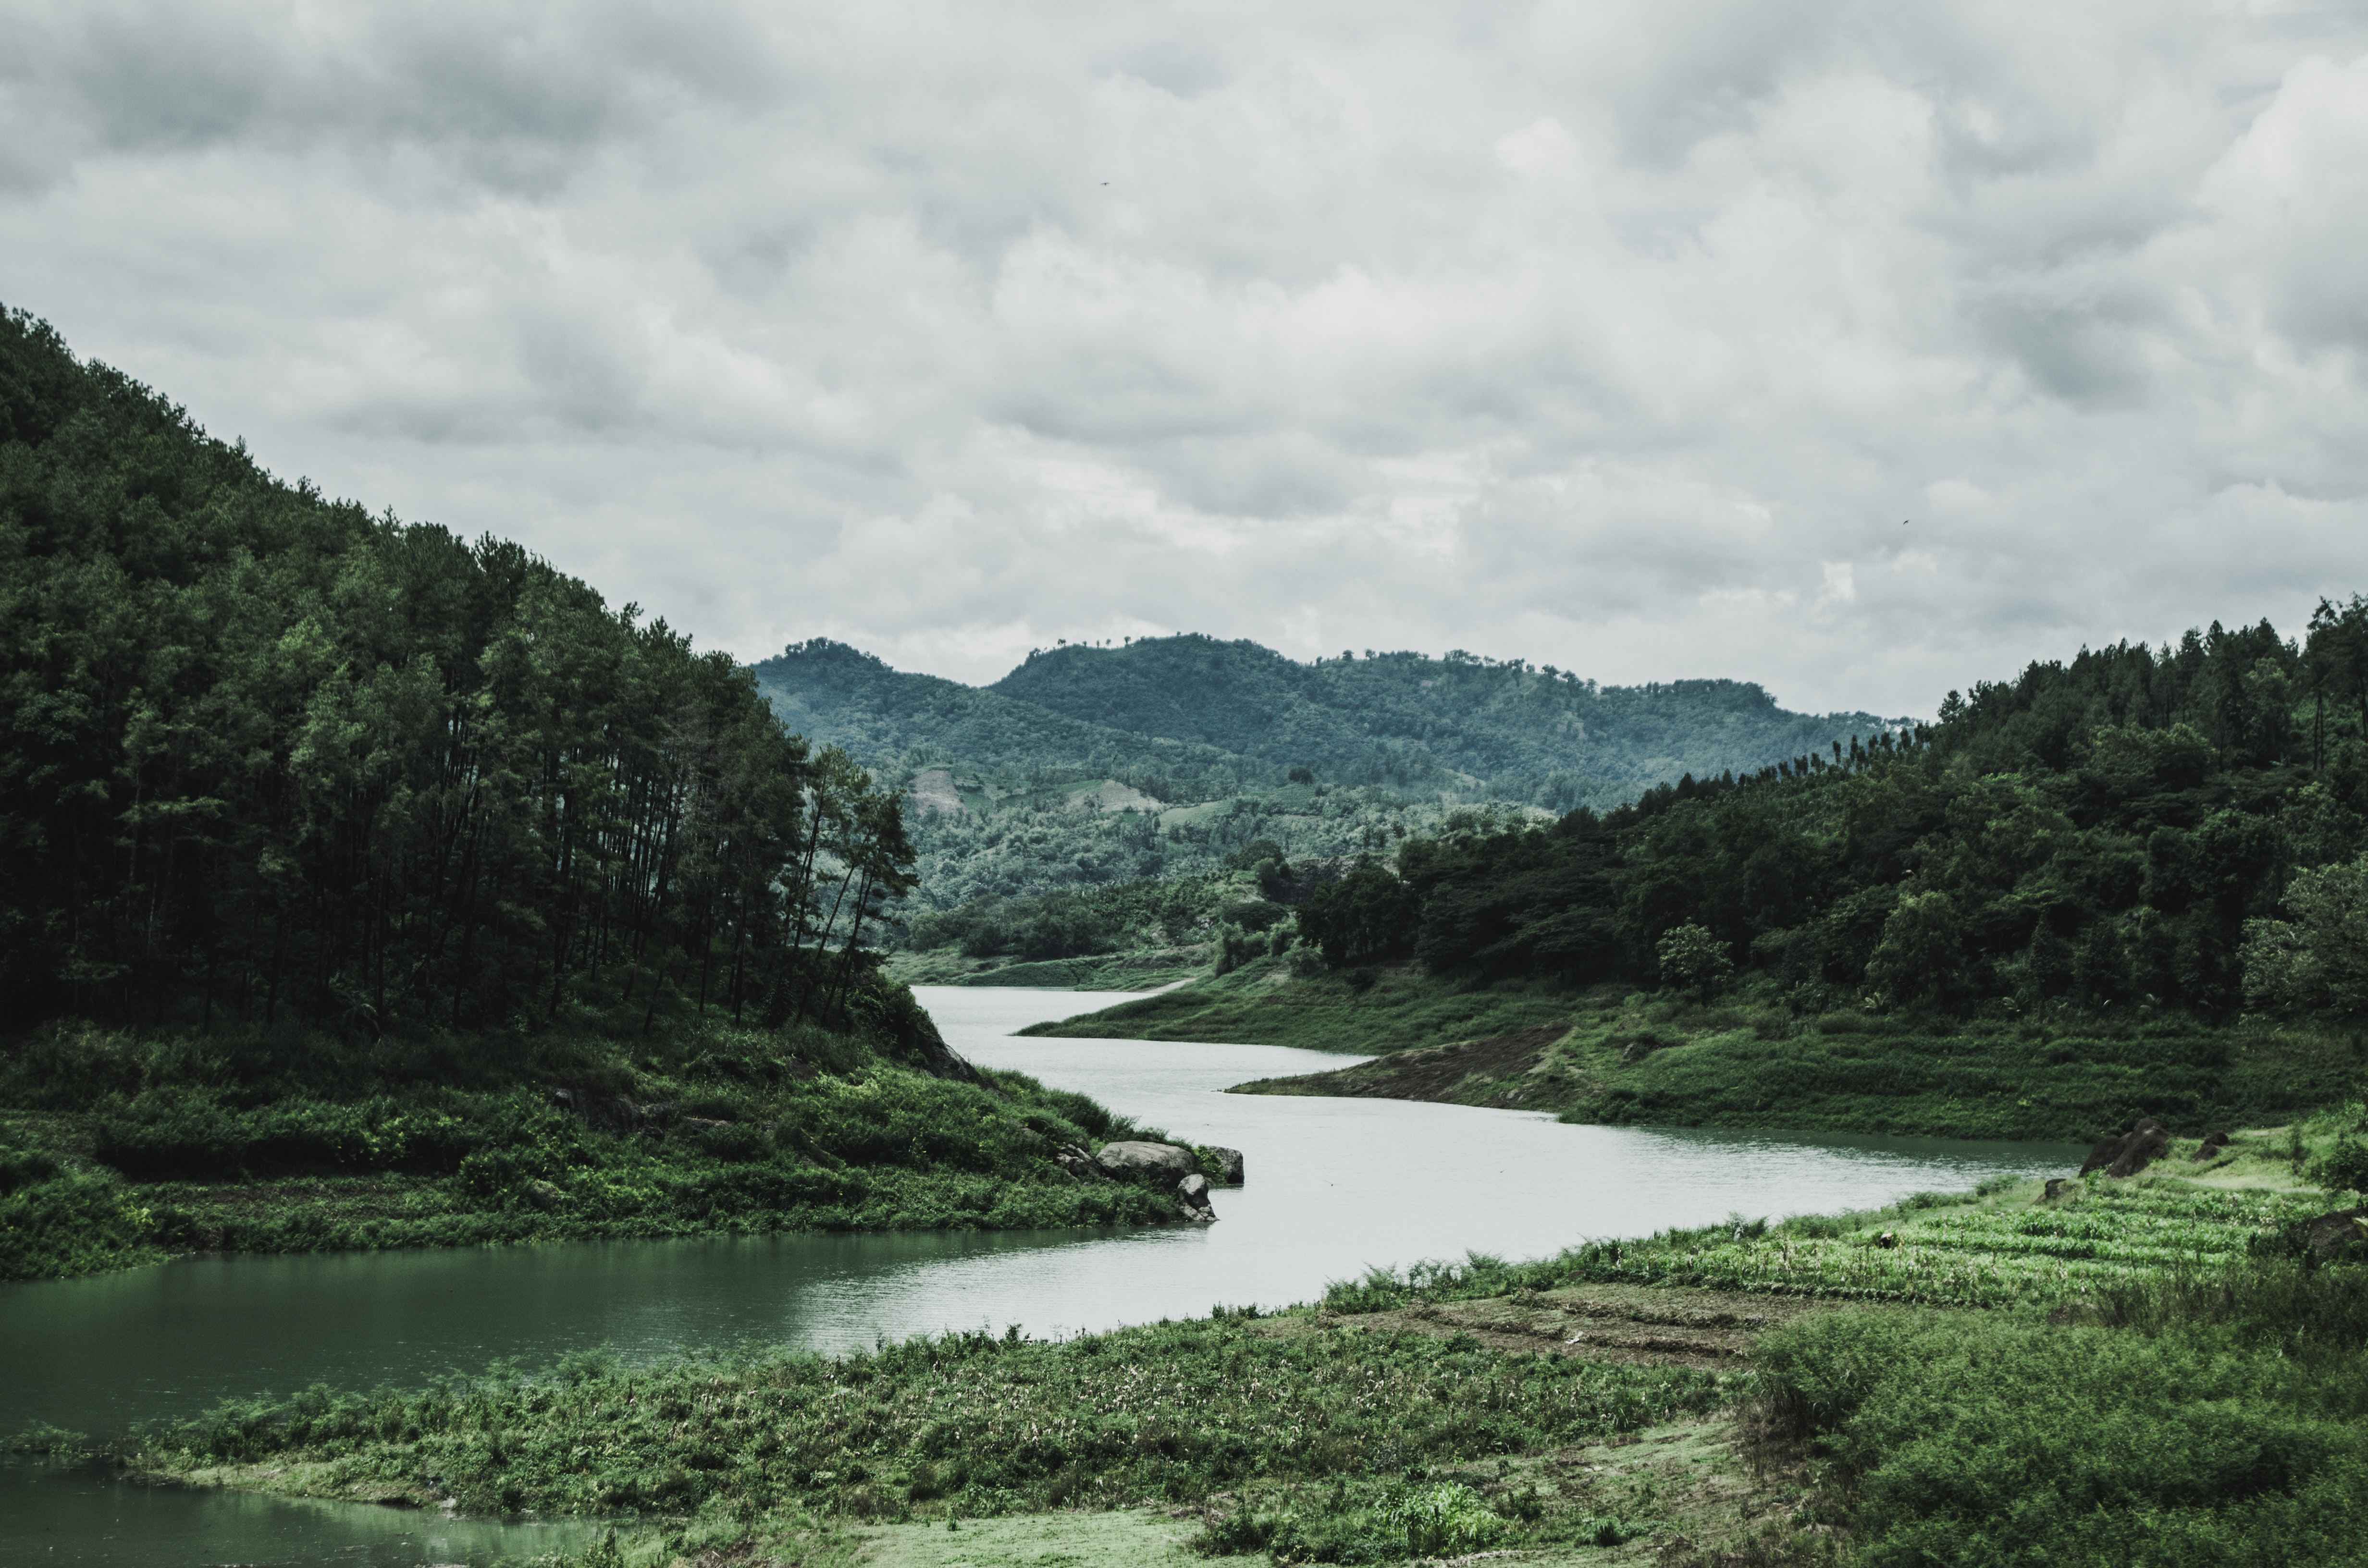
\includegraphics[width=\textwidth]{images/pexels-rido-alwarno-1034887.jpg}
            \caption{A river.}
            \label{fig:01_river}
        \end{subfigure}
        \hfill
        \begin{subfigure}[b]{0.45\textwidth}
            \centering
            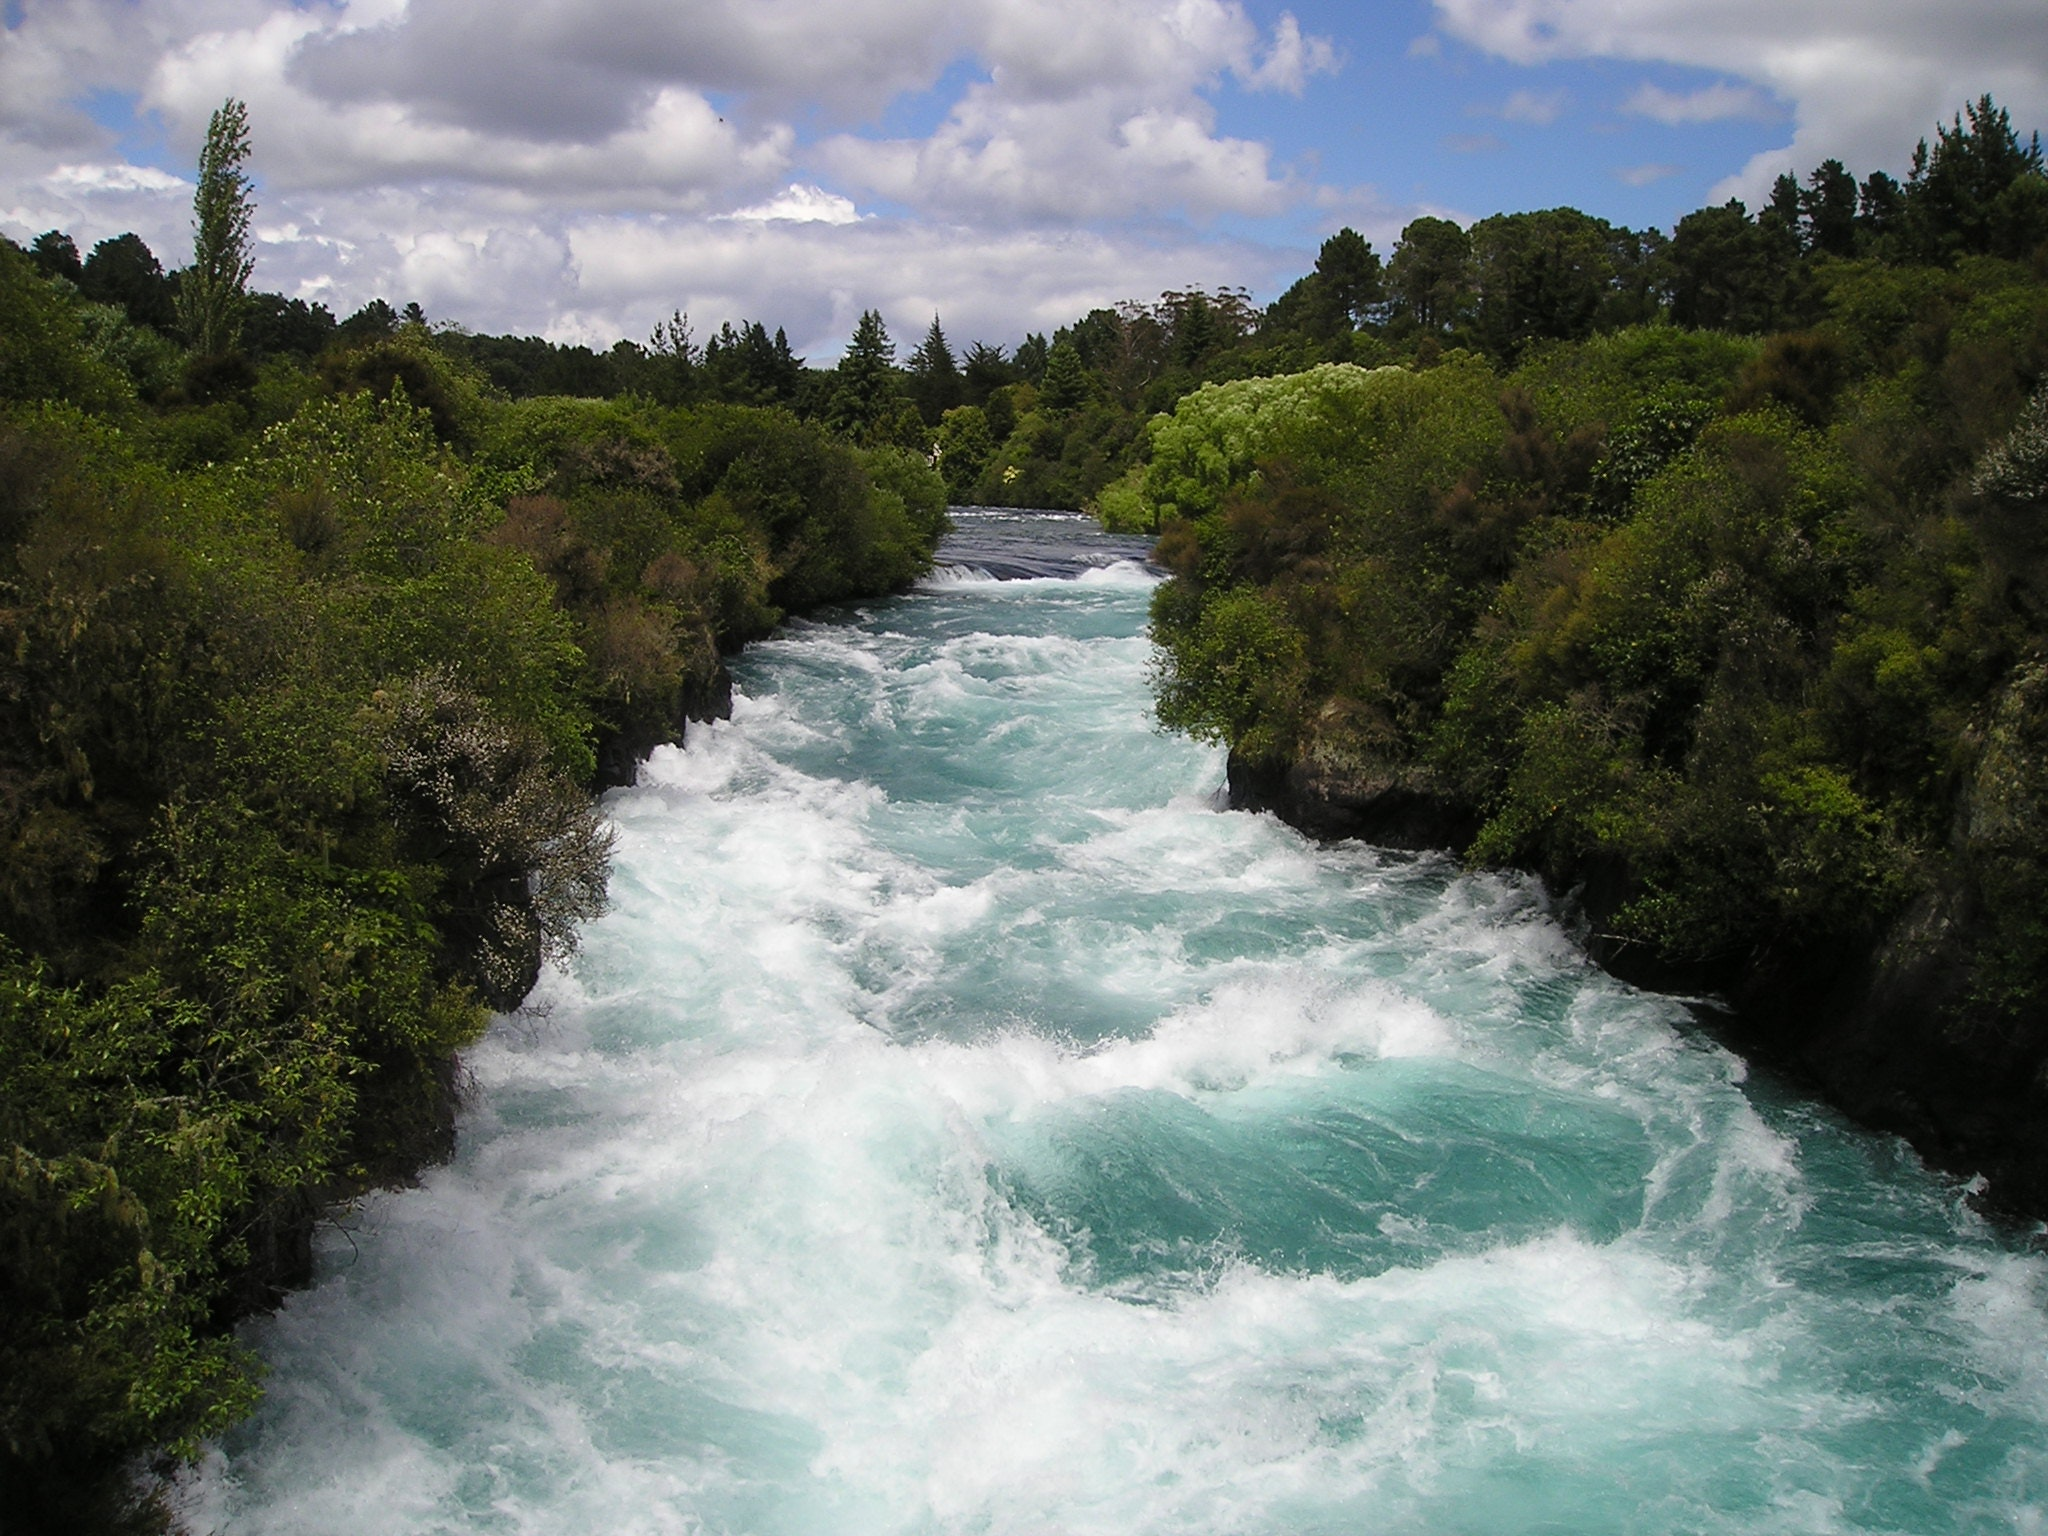
\includegraphics[width=\textwidth]{images/pexels-pixabay-2438.jpg}
            \caption{An angry river.}
            \label{fig:01_angry_river}
        \end{subfigure}
        \caption{Natural wave phenomena.}
        \label{fig:rivers}
    \end{figure}
\end{frame}
\begin{frame}
    \frametitle{Background}

    We explore this question in the context of the 1D Shallow-Water Equations (SWE).
    \bigskip

    \pause 
    The SWEs are a system of hyperbolic partial differential equations (PDE) which represent a simplified model of fluid
    flow.

    \bigskip
    \pause
    These equations are derived from the Navier-Stokes equations where the horizontal length scale is
    much greater than the vertical length scale (e.g., oceanic modeling, river flow, flood waves, etc.).
\end{frame}
\begin{frame}
    \frametitle{The Equations}

    \ \\
    \setlength{\belowcaptionskip}{-20pt}
    \begin{figure}
        \centering
        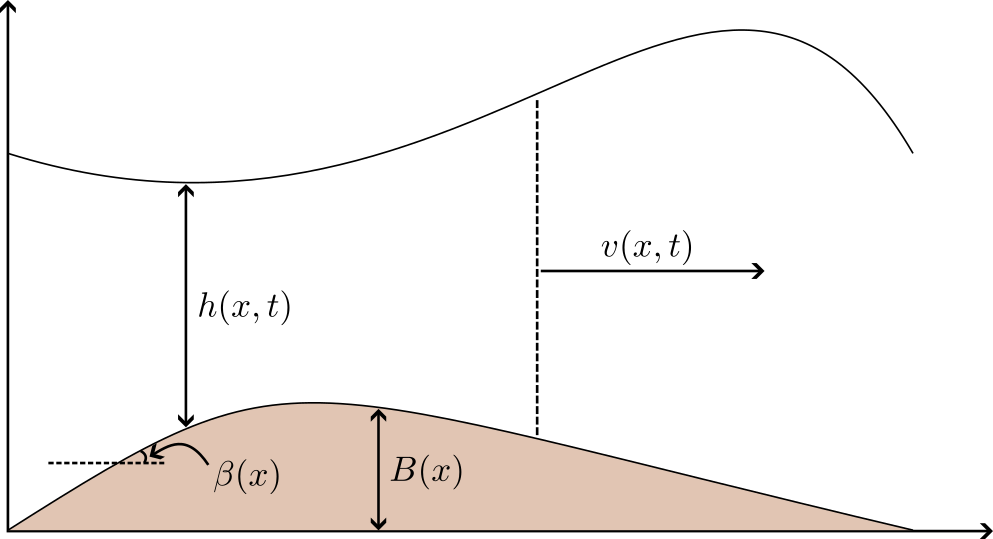
\includegraphics[width=0.7\textwidth]{images/swe_diagram.png}
        \caption{SWE Formulation. $\tan{\alpha} = B_x$}
        \label{fig:03_swe_diagram}
    \end{figure}

    \begin{align*}
           & h_t + (h v)_x = 0 & \text{(mass)} \\
           & (h v)_t + \left[ hv^2 + \frac{1}{2} g h^2 \cos{(\alpha)} \right]_x - g h \sin{(\alpha)} + C_f v^2 = 0 & \text{(momentum)}
    \end{align*}
\end{frame}
\begin{frame}
    \frametitle{Methodology: Approximation}

    Given some initial state (boundary conditions and initial conditions) of the system, we'd like to find out how
    $h(x, t)$, $v(x, t)$, and $\beta(x)$ evolve over space and, where applicable, time.

    \bigskip
    \pause
    Systems like this are rarely solveable analytically, so we utilize a numerical approach. 

    \bigskip
    \pause
    One such approach is to create an analytic approximation function $\mathcal{N}: \mathbb{R}^2 \to \mathbb{R}^3$ to the true solution so that:

    $$
    \mathcal{N}(x, t) = \begin{pmatrix*}
        \mathcal{N}_h \\
        \mathcal{N}_v \\
        \mathcal{N}_\beta 
    \end{pmatrix*} \approx \begin{pmatrix*}
        h \\
        v \\
        \beta
    \end{pmatrix*}.
    $$
\end{frame}
\begin{frame}
    \frametitle{Methodology: Residual}

    We are almost ready to frame this as an unconstrained optimization problem. To do so, we substitute our approximation 
    function into the SWE system. 

    \bigskip
    \pause

    Since we're only approximating the solution, we expect there to be some amount ``left over", which we call the 
    \textit{residual} and denote $R$. 
    
    \bigskip
    \pause

    The first equation in the system 
    
    $$
    h_t + (hv)_x = 0
    $$
    
    yields the residual term associated with conservation of mass:

    $$
    \left( \mathcal{N}_h \right)_t + \left( \mathcal{N}_h \mathcal{N}_v \right)_x = R_{mass}(x, t).
    $$

    \bigskip
    \pause

    The residual term associated with the momentum is similarly obtained from the second equation, which we denote 
    $R_{momentum}$.
\end{frame}
\begin{frame}
    \frametitle{Methodology: Optimization}

    We find the best approximation to the true solution by solving the non-linear unconstrained minimization problem:

    $$
    \min_{\mathcal{N}} {\lVert R_{mass} \rVert + \lVert R_{momentum} \rVert}.
    $$

    \bigskip
    \pause

    At this point, we have a well-defined optimization problem, but we still need to decide what our approximation 
    function $\mathcal{N}$ "looks like". 

    \bigskip
    \pause

    Ideally, we'd like a function which can modified to minimize the PDE residual via existing optimization algorithms.
\end{frame}
\begin{frame}
    \frametitle{Implementation}

    Neural networks fit the bill! What are they?

    \medskip
    \pause

    A (feedforward) neural network is an affine composition (e.g., $f(g(x)) = m g(x) + b$) of multivariate ``squashing''
    functions, such as the sigmoid or hyperbolic tangent functions. 
   
    \bigskip
    \pause More importantly, for particular choices of ``squashing" functions, neural networks are:
    \bigskip

    \begin{itemize}
        \setlength\itemsep{1.5em}
        \item Universal function approximators (for Borel-measurable functions over compact domains).
        \item Infinitely differentiable (analytic).
        \item Trainable via gradient descent (by modifying the coefficients $m$ and $b$ of the affine maps).
    \end{itemize}
\end{frame}
\begin{frame}
    \frametitle{Optimization Algorithms}

    Since neural networks have a \textit{lot} of parameters to train, we use stochastic gradient descent variations to 
    make the training process possible on modern hardware.

    \bigskip
    \pause

    In stochastic gradient descent, we use random subsets of the training data to compute the gradient of the residual
    in place of the entire set.

    \bigskip
    \pause

    \textbf{Adaptive Moment Estimation (Adam)}
    \ \\
    \bigskip

    [\textbf{TODO:} Describe Hessian approximation ]

    \pause
    \bigskip

    \textbf{Limited-Memory BFGS (L-BFGS)}
    \ \\
    \bigskip
    [\textbf{TODO:} Describe Hessian approximation ]
\end{frame}
\begin{frame}
    \frametitle{Optimization Algorithms}
    \textbf{Adaptive Moment Estimation (Adam)}
    
    \bigskip
    Adam SGD approximates the full gradient of the objective function over the computational domain by numerically computing the gradient over a random subset. An update has the form
    \[x_{k+1} = x_k - \alpha_i \nabla f_i(x_k)\]
    where $f_i$ is the objective function sampled at the $i^{\text{th}}$ domain point and $\alpha_i$ is a variable learning rate based on the computed gradient
    from previous iterations.

    \pause
    \bigskip

    \textbf{Limited-Memory BFGS (L-BFGS)}
    
    \bigskip
    L-BFGS approximates the inverse Hessian of the objective function by a recursive algorithm that utilizes at most $m$ past updates of the gradient and data values.
\end{frame}
\begin{frame}
    \frametitle{Methodology: Inference}

    In Appendix A, we successfully solve the classical homogeneous system with fluid flow over a flat surface.

    \bigskip
    \pause
    
    Let's try something more difficult. Based on some experimental height and velocity measurements, could a neural 
    network ``see'' under the fluid surface to infer the bathymetry function $\beta(x)$ when it's not known in advance?

    \bigskip
    \pause

    For this problem, we'll choose our neural network to be a mapping from 
    $\mathbb{R}^2 \to \mathbb{R}^3$:

    $$
    \mathcal{N}(x, t) = \begin{pmatrix*}
        \mathcal{N}_h \\
        \mathcal{N}_v \\
        \mathcal{N}_{\beta}
    \end{pmatrix*} \approx \begin{pmatrix*}
        h \\
        v \\
        \beta
    \end{pmatrix*}.
    $$
\end{frame}
\begin{frame}
    \frametitle{Methodology: Inference}

    To account for the new experimental data, we'll also add a new residual term $R_{data}$ to ensure that our neural
    network is consistent with these measurements:

    $$
    R_{data} = \frac{1}{N} \sum\limits_{i=1}^N \left( \mathcal{N}_h (x_i, t_i) - h_i \right)^2 
                                             + \left( \mathcal{N}_v (x_i, t_i) - v_i \right)^2.
    $$

    \bigskip
    \pause
    Our new optimization problem then becomes

    $$
    \min_{\mathcal{N}} {\lVert R_{mass} \rVert + \lVert R_{momentum} \rVert + \lVert R_{data} \rVert}.
    $$

    We call the resulting neural network solution a \textit{physics-informed neural network} (PINN).
\end{frame}
\begin{frame}
    \frametitle{Results: Inhomogeneous System}

    We apply this methodology to the inhomogeneous system, where our bathymetry function 
    $\beta(x)$ is given by

    $$
    B(x) = -\frac{1}{4} + \frac{1}{4} \cos{\left( \frac{\pi x}{5} \right)}.
    $$
    
    We impose periodic boundary conditions, no initial velocity, and sinusoidal initial condition

    $$
    h(x, 0) = \frac{1}{2} + \frac{2}{5} \sin{\left( \frac{\pi x}{10} \right)}
    $$

    where $x \in [0, 10]$ and $t \in [0, 4]$.

    \medskip
    \pause

    After 100,000 Adam iterations and 16,000 L-BFGS iterations, we obtain a mean PDE residual (over a randomly sampled 
    subset $\Omega$ of our domain) of 
    
    $$
    \lVert R(\Omega) \rVert_2 = 0.004952.
    $$
\end{frame}
\begin{frame}
    \frametitle{Results: Wave Height}

    \begin{figure}
        \centering
        \begin{subfigure}[b]{0.45\textwidth}
            \centering
            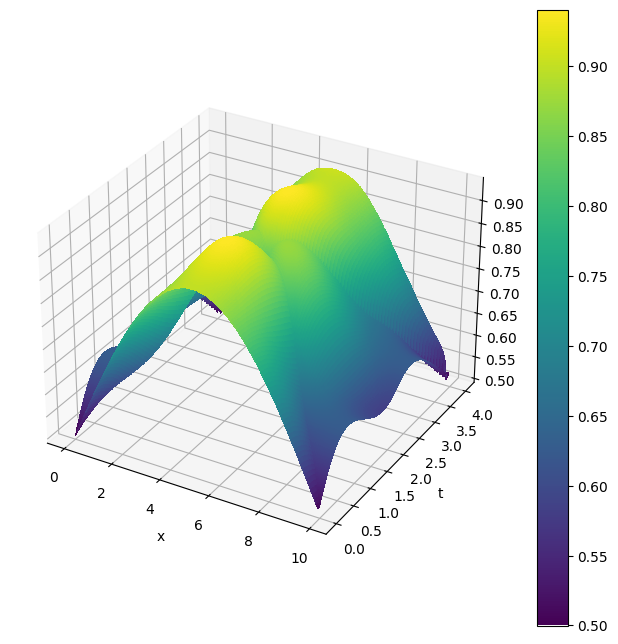
\includegraphics[width=\textwidth]{images/inhomogeneous_swe_pseudospectral_height.png}
            \caption{Reference solution}
            \label{fig:15_inhomogeneous_pseudospectral_swe_height}
        \end{subfigure}
        \hfill
        \begin{subfigure}[b]{0.45\textwidth}
            \centering
            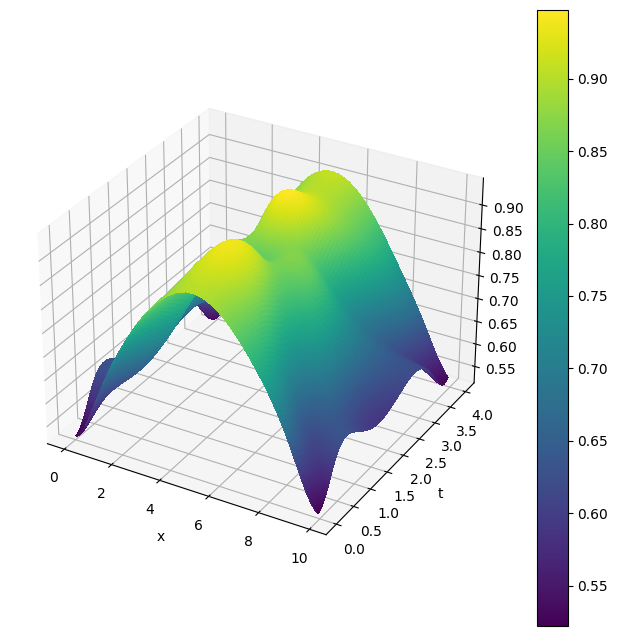
\includegraphics[width=\textwidth]{images/inhomogeneous_swe_pinn_height.png}
            \caption{PINN solution}
            \label{fig:15_inhomogeneous_pinn_swe_height}
        \end{subfigure}
        \caption{Wave height (inhomogeneous)}
        \label{fig:15_inhomogeneous_wave_height}
    \end{figure}
\end{frame}
\begin{frame}
    \frametitle{Results: Wave Velocity}

    \begin{figure}
        \centering
        \begin{subfigure}[b]{0.45\textwidth}
            \centering
            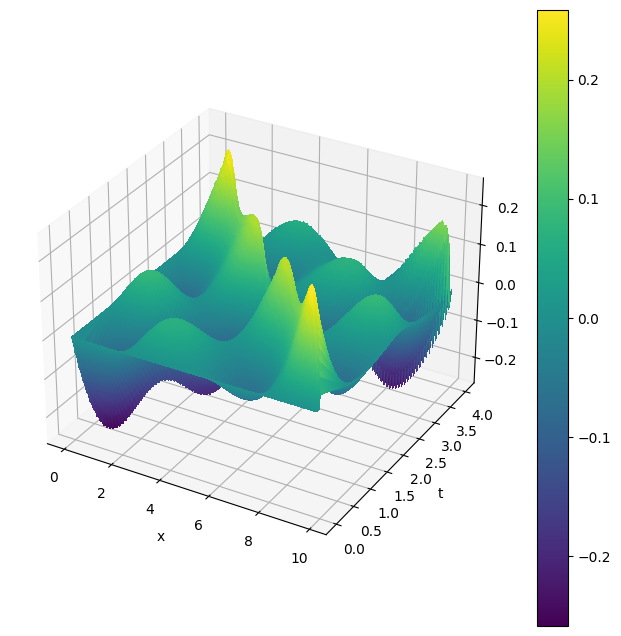
\includegraphics[width=\textwidth]{images/inhomogeneous_swe_pseudospectral_velocity.png}
            \caption{Reference solution}
            \label{fig:16_inhomogeneous_pseudospectral_swe_velocity}
        \end{subfigure}
        \hfill
        \begin{subfigure}[b]{0.45\textwidth}
            \centering
            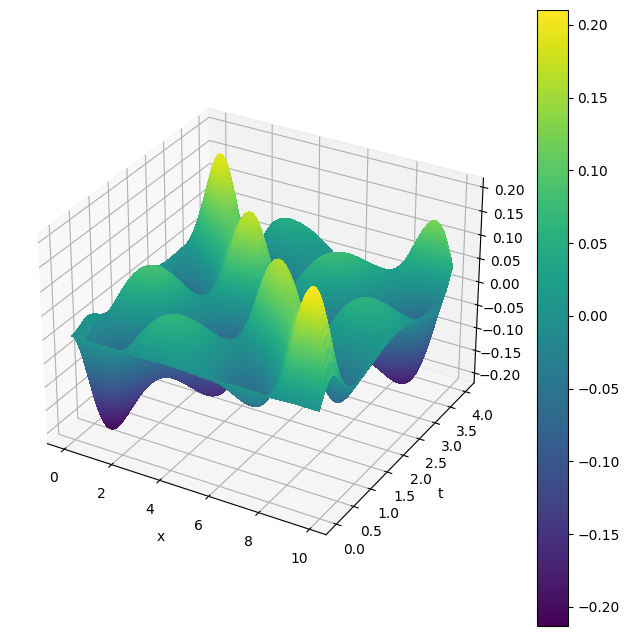
\includegraphics[width=\textwidth]{images/inhomogeneous_swe_pinn_velocity.png}
            \caption{PINN solution}
            \label{fig:16_inhomogeneous_pinn_swe_velocity}
        \end{subfigure}
        \caption{Wave velocity (inhomogeneous)}
        \label{fig:16_inhomogeneous_wave_velocity}
    \end{figure}
\end{frame}
\begin{frame}
    \frametitle{Results: Inferred Bathymetry}

    \begin{figure}
        \centering
        \begin{subfigure}[b]{0.45\textwidth}
            \centering
            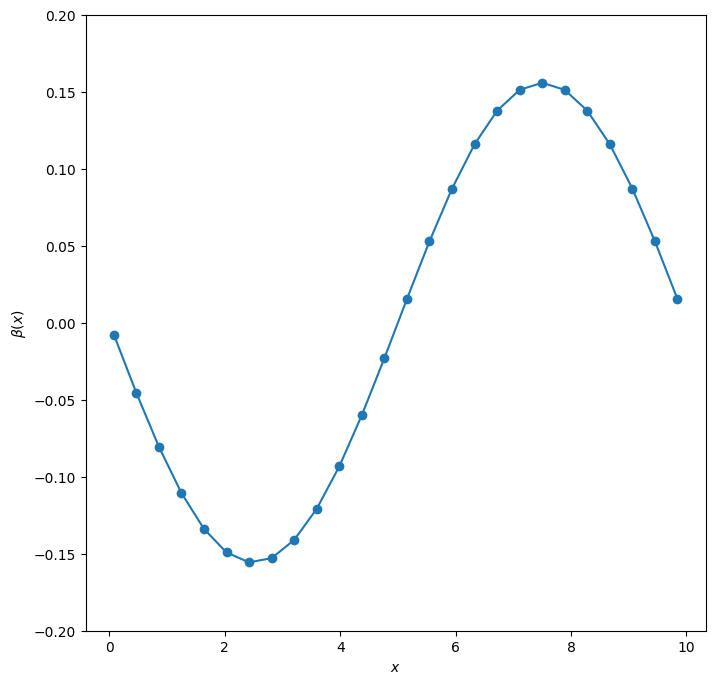
\includegraphics[width=\textwidth]{images/inhomogeneous_swe_pseudospectral_bathymetry_angle.png}
            \caption{Reference solution}
            \label{fig:17_inhomogeneous_pseudospectral_swe_bathymetry}
        \end{subfigure}
        \hfill
        \begin{subfigure}[b]{0.45\textwidth}
            \centering
            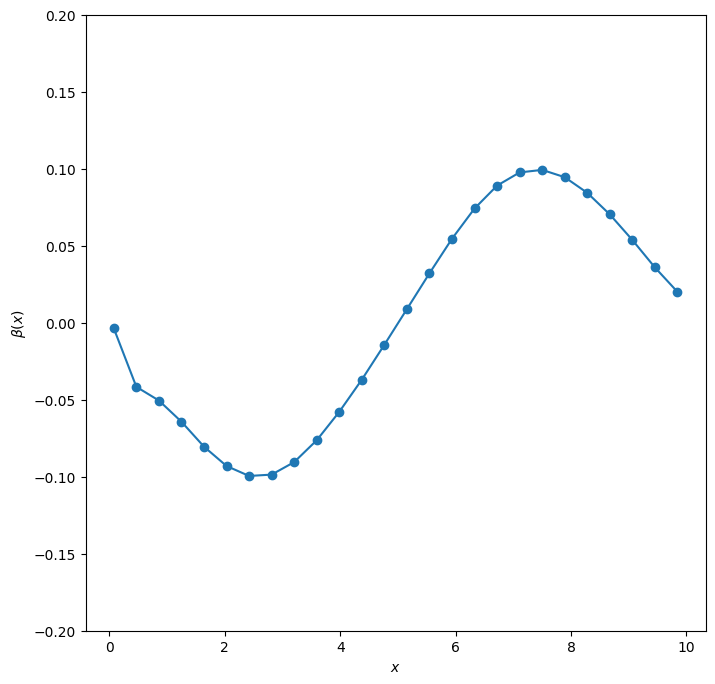
\includegraphics[width=\textwidth]{images/inhomogeneous_swe_pinn_bathymetry_angle.png}
            \caption{PINN solution}
            \label{fig:17_inhomogeneous_pinn_swe_bathymetry}
        \end{subfigure}
        \caption{Bathymetry (inhomogeneous)}
        \label{fig:17_inhomogeneous_bathymetry}
    \end{figure}
\end{frame}
\begin{frame}
    \frametitle{Conclusions}

    \begin{itemize}[<+->]
        \setlength\itemsep{2em}
        \item Neural networks are capable of solving classical PDE problems (i.e., with BCs and ICs).
        \item PINNs can incorporate experimental observations into PDE residual minimization.
        \item Our PINN correctly identified the bathymetry function shape and scale from experimental observations of 
              wave height and velocity alone.
        \item Our results validate this approach and leave room for future work.
    \end{itemize}
\end{frame}
\begin{frame}[c]
    \begin{center}
        \Huge Thank you!
    \end{center}
\end{frame}
\begin{frame}[c]
    \begin{center}
        \Huge Questions?
    \end{center}
\end{frame}

% Appendices
\begin{frame}
    \frametitle{Appendix A: Homogeneous Forward Problem}

    We apply the PINN approach to the homogeneous system, where friction is negligible and our bathymetry function 
    $\beta(x)$ is zero so that fluid flows over a flat surface.  We impose periodic boundary conditions, no initial 
    velocity, and the following sinusoidal initial condition

    $$
    h(x, 0) = 2 + \sin{\left( \frac{\pi x}{100} \right)}
    $$

    where $x \in [0, 200]$ and $t \in [0, 15]$.

    \medskip
    \pause

    After 50,000 Adam iterations and 12,000 L-BFGS iterations, we obtain a mean PDE residual (over a randomly sampled 
    subset $\Omega$ of our domain) of 
    
    $$
    \lVert R(\Omega) \rVert_2 = 0.006090.
    $$
\end{frame}
\begin{frame}
    \frametitle{Appendix A: Homogeneous Forward Problem}

    \begin{figure}
        \centering
        \begin{subfigure}[b]{0.45\textwidth}
            \centering
            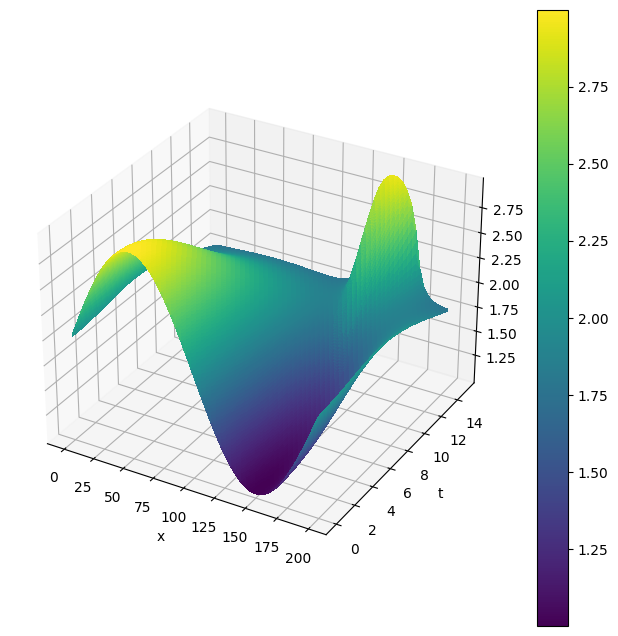
\includegraphics[width=\textwidth]{images/homogeneous_swe_pseudospectral_height.png}
            \caption{Reference solution}
            \label{fig:10_homogeneous_pseudospectral_swe_height}
        \end{subfigure}
        \hfill
        \begin{subfigure}[b]{0.45\textwidth}
            \centering
            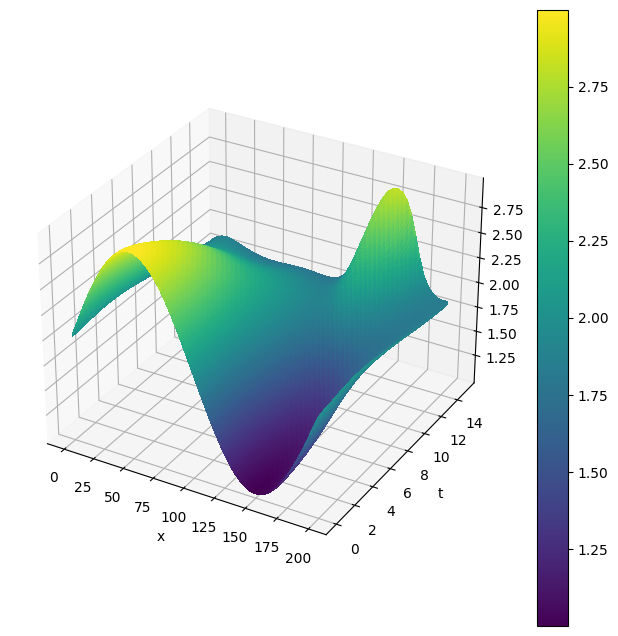
\includegraphics[width=\textwidth]{images/homogeneous_swe_pinn_height.png}
            \caption{PINN solution}
            \label{fig:10_homogeneous_pinn_swe_height}
        \end{subfigure}
        \caption{Wave height (homogeneous)}
        \label{fig:10_homogeneous_wave_height}
    \end{figure}
\end{frame}
\begin{frame}
    \frametitle{Appendix A: Homogeneous Forward Problem}

    \begin{figure}
        \centering
        \begin{subfigure}[b]{0.45\textwidth}
            \centering
            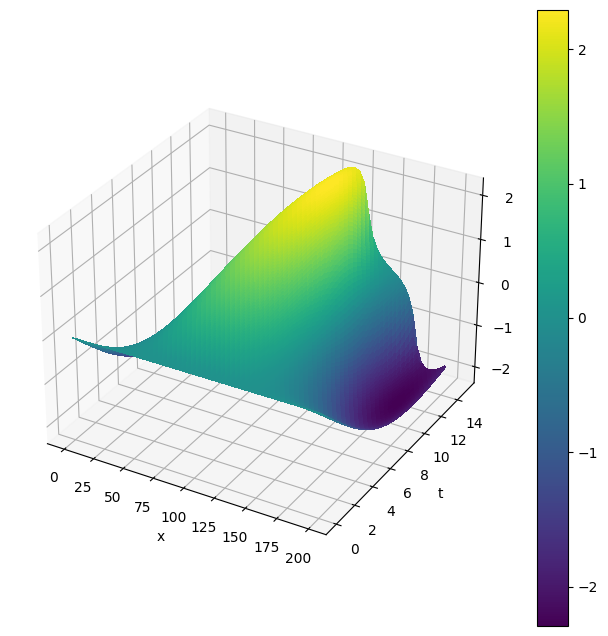
\includegraphics[width=\textwidth]{images/homogeneous_swe_pseudospectral_velocity.png}
            \caption{Reference solution}
            \label{fig:10_homogeneous_pseudospectral_swe_velocity}
        \end{subfigure}
        \hfill
        \begin{subfigure}[b]{0.45\textwidth}
            \centering
            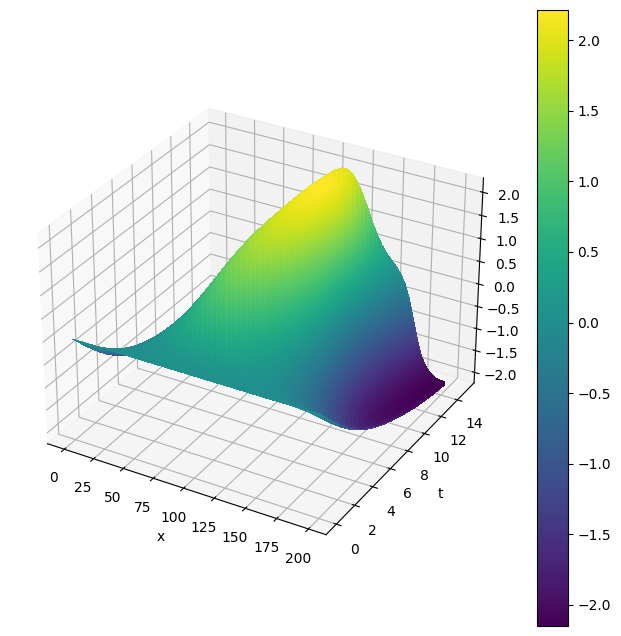
\includegraphics[width=\textwidth]{images/homogeneous_swe_pinn_velocity.png}
            \caption{PINN solution}
            \label{fig:10_homogeneous_pinn_swe_velocity}
        \end{subfigure}
        \caption{Wave velocity (homogeneous)}
        \label{fig:11_homogeneous_wave_velocity}
    \end{figure}
\end{frame}

\end{document}
